% !TEX root = ../thesis.tex

\chapter{Analytická časť}\label{ch:current-state}

\section{Klasifikácia objektov}

Pod názvom klasifikácia objektov môžeme chápať úlohu, ktorá identifikuje a kategorizuje objekty v obrázku s vopred definovanými triedami.
Klasifikácia objektov je typicky vykonávaná technológiami strojového učenia, kde model je trenovaný na vybranej dátovej sade obrázkov a ich priradenie do označených tried.
Trenovací model môže byť použitý na klasifikovanie nových obrázkov priradením označenia triedy na základe ich naučených vlasností.
Použitie klasifikácie objektov je zahrnuté napr. pri rozpoznávaní dopravných značiek alebo identifikáciu rastliny na obrázku. \cite{kili}

\begin{figure}[H]
    \centering
    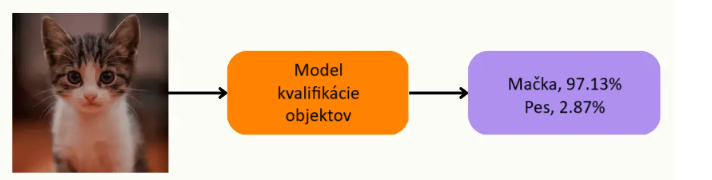
\includegraphics[width=1\linewidth]{figures/OCmodel.png}
    \caption{Zreťazenie klasifikácie objektov \label{OCmodel}}
    \label{fig:enter-label}
\end{figure}

\section{Detekcia objektov}

Detekcia objektov je z pohľadu počítača úloha, ktorá identifikuje a lokalizuje objekty na základe preddefinovaných triedach vo vstupných obrázkov.
S vývojom neurónových sietí, detekcia objektov dosiahla veľmi sľubné výsledky.
Existuje pár modelov a algoritmov ako sú \acrfull{rcnn}, rýchlejší \acrshort{rcnn}, \acrfull{yolo} a \acrfull{ssd}, ktoré boli vyvinuté na detekciu objektov.
Tieto algoritmy a modely sa používajp v rôznych aplikáciách, ako je samojazdiace autá, sledovacie systémy a sledovanie objektov. \cite{kili}

\begin{figure}[H]
    \centering
    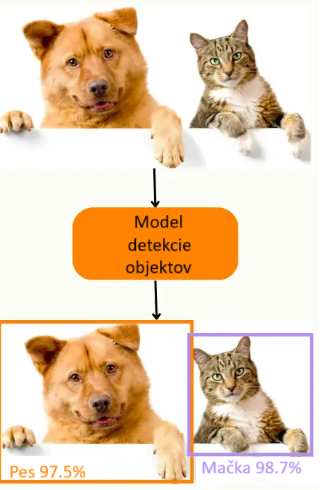
\includegraphics[width=0.45\linewidth]{figures/ODmodel.png}
    \caption{Zreťazenie detekcie objektov \label{ODmodel}}
    \label{fig:enter-label}
\end{figure}

\section{\acrshort{yolo}}

\acrshort{yolo} je algoritmus detekcie objektov v reálnom čase, vyvinutý v roku 2015 dvojicou autorov Joseph Redmon a Ali Farhadi.
Ide o jednostupňový detektor objektov, ktorý využíva konvolučnú neurónovú sieť (\acrshort{cnn}) na prepovedanie ohraničujúcich políčok a prevdepodobností tried objektov vo vstupných obrázkoch.

Algoritmus \acrshort{yolo} rozdeľuje vstupný obrázok na mriežku buniek a pre každú bunku predpovedá pravdepodobnosť prítomnosti objektu a súradnice ohraničujúceho rámčeka objektu a prepovedá tiež triedu objektu.
Na rozdiel od dvojstupňovových detektorov objektov, ako je \acrshort{rcnn} a jeho variantov, \acrshort{yolo} spracováva celý obraz v jednom priechode, vďaka čomu je rýchlejší a efektívnejší.

\acrshort{yolo} bolo vyvinuté v niekoľkých verziách od \acrshort{yolo}v1 až po najnovšie \acrshort{yolo}v12. Každá verzia bola postavená na predchádzajúcej verzii s vylepšenými funkciami, ako je vylepšená presnosť, rýchlejšie spracovanie a lepšia manipulácia s malými predmetmi.

\acrshort{yolo} je široko používaný v rôznych aplikáciach, ako sú samoriadiace autá a sledovacie systémy.
Je tiež široko používaný na úlohy detekcie objektov v reálnom čase, ako je analýza videa v reálnom čase a video dohľad v reálnom čase. \cite{kili}

Ľavá časť obrázku vykresľuje pomer strednej priemernej presnosti ku odozve, ktoré sú zoradené podľa veľkosti od nano (n) až po x (xlarge),
kde druhá časť obrázku znázorňuje pomer strednej priemernej presnosti ku \acrfull{flops} a taktiež zoradené podľa veľkosti od nano (n) až po x (xlarge).

\begin{figure}[H]
    \centering
    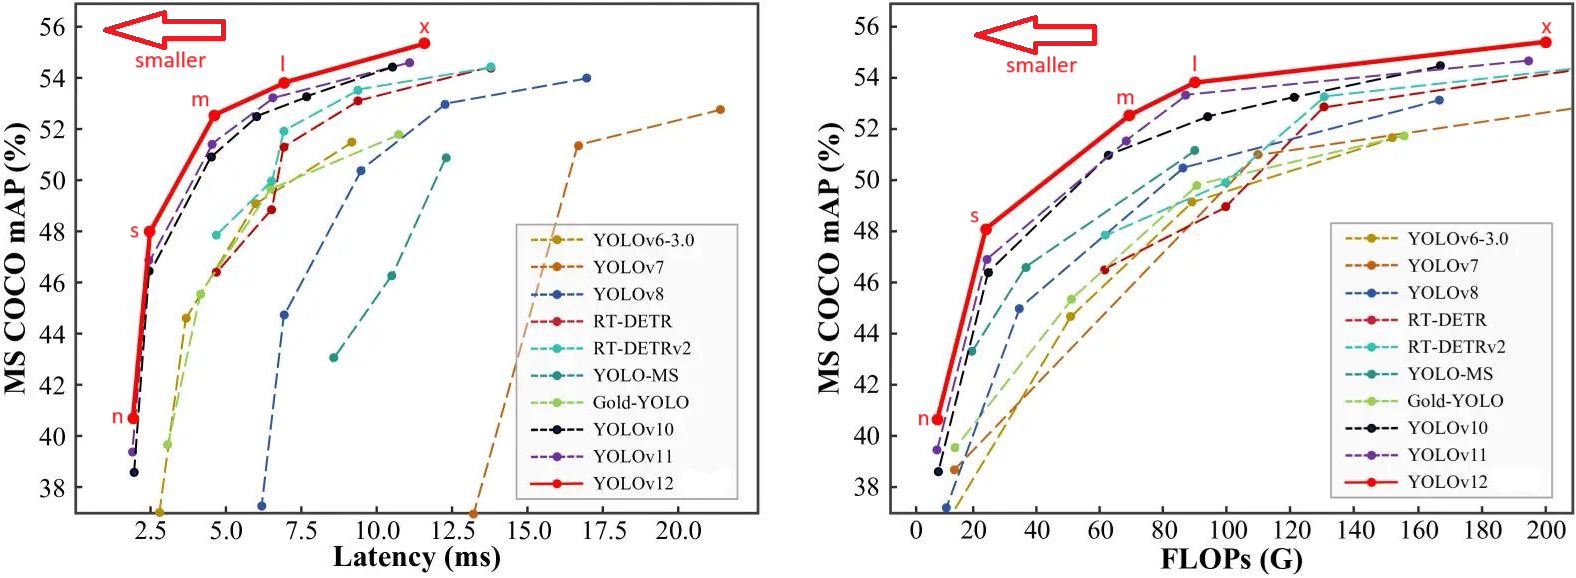
\includegraphics[width=1\linewidth]{figures/yolo.png}
    \caption{Porovnanie s ďalšimi známymi metódami pokiaľ ide o kompromisy latencie-presnosť (vľavo) a FLOP-presnosť (vpravo) \label{yolo}}
    \label{fig:enter-label}
\end{figure}

\subsubsection{Princíp \acrshort{yolo} algoritmu}

Základný princíp \acrshort{yolo} spočína v rozdelení vstupného obrázka na mriežku buniek a pre každú bunku prepovedá pravdepodobnosť prítomnosti objektu a súradnice ohraničujúceho rámčeka objektu.
Proces \acrshort{yolo} sa môže rozdeliť do niekoľkých krokov:

\begin{enumerate}

    \item Vstupný obrázok sa odovzdáva cez \acrshort{cnn}, aby sa z obrázka extrahovali prvky.
    \item Prvky sa potom prechádzajú sériou plne prepojených vrstiev, ktoré predpovedajú pravdepodobnosť tried a súradnice ohraničujúceho rámčeka.
    \item Obrázok je rozdelený na mriežku buniek a každá bunka je zodpovedná za predpovedanie množiny ohraničujúcich políčok a pravdepodobností tried.
    \item Výstupom siete je súbor ohraničujúcich rámčekov a pravdepodobností tried pre každú bunku.
    \item Ohraničujúce rámčeky sa potom filtrujú pomocou algoritmu následného spracovania nazývaného non-max suppression, aby sa odstránili prekrývajúce sa rámčeky a aby sa vybral rámček s najvyššou prevdepodobnosťou.
    \item Konečným výstupom je sada predpokladaných ohraničujúcich rámčekov a označaní tried pre každý objekt na obrázku. \cite{kili}

\end{enumerate}

\section{\acrfull{mec}}

\acrlong{mec} alebo \acrshort{mec} architektúra, ktorá umožňuje poskytovateľom výpočtových, sieťových a mobilných služieb presunúť niektoré výpočtové a cloudové procesy na okraj sieťového prostredia, čím sa dosiahne lepší výkon, latencia a bezpečnosť.
\acrfull{mec} je myšlienka alebo koncept vyvinutý Európskym inštitútom pre telekomunikačné normy (ETSI).
Na rozdiel od dátového centra poskytuje táto sieťová architektúra služby požadované používateľmi a operáciae cloud computingu na okraji siete, ktorý je bližšie ku koncovým používateľom. \cite{mec}

\begin{figure}[H]
    \centering
    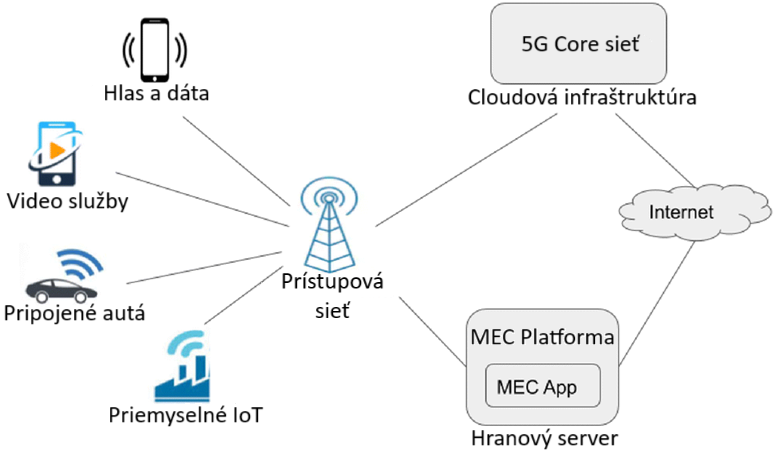
\includegraphics[width=1\linewidth]{figures/MEC.png}
    \caption{\acrfull{mec} architektúra \label{mec}}
    \label{fig:enter-label}
\end{figure}

Význam \acrshort{mec} možno rozdeliť takto:

\begin{itemize}

    \item Viacnásobný prístup (Multi-Access) - Viacnásobný prístup umožňuje systému \acrshort{mec} poskytovať bezproblémový zážitok zákazníkom pristupujúcim k sieti prostredníctvom technológie podľa vlastného výberu.
    \item Hrana (EDGE) - Premiestnenie sieťových operácií a aplikácií na okraj siete umožňuje mimoriadne nízku latenciu.
    \item Výpočtová technika (Computing) - Výpočtové možnosti siete sú rozložené smerom k hrane siete.

\end{itemize}

Medzi kľúčové vlastnosti \acrshort{mec} patria:

\begin{itemize}

    \item Tesná blízkosť ku koncovému užívateľovi
    \item Nízka latencia dátového prenosu
    \item Vhodnosť pre aplikácie v reálnom čase
    \item Neprerušované prevádzkové schopnosti
    \item Vzájomná komunikácia s existujúcimi aplikáciami
    \item Väčšia miera virtualizácie \cite{mec}

\end{itemize}